% ============================================================================
% Chapter 4 — Performance Evaluation
% Numbers below are the measured classical-baseline results on the held-out test
% split (4,870 documents). Fill the XLM-RoBERTa / BanglaBERT rows after running
% notebooks/02 on Colab (reports/xlmr_metrics.json, reports/banglabert_metrics.json).
% ============================================================================
\chapter{Performance Evaluation}
\label{ch:results}

\section{Simulation or Testbed Environment}
The classical baselines were trained and evaluated on CPU; the transformer models
were fine-tuned on a single GPU (Google Colab, NVIDIA T4). The software stack
comprises Python~3, scikit-learn for the classical models, and PyTorch with the
HuggingFace Transformers library for the transformer models. The assembled corpus
contains $32{,}463$ documents, partitioned into stratified train, validation, and
test splits of $22{,}724$, $4{,}869$, and $4{,}870$ documents respectively. All
models are evaluated on the same held-out test split.

\section{Performance Metrics}
The system is evaluated using standard multi-class classification metrics:
\textbf{accuracy}, and macro-averaged \textbf{precision}, \textbf{recall}, and
\textbf{F1-score}. Macro-averaging weights each class equally and is therefore
the primary metric, given the class imbalance in the corpus. Per-class F1 and a
confusion matrix are reported to expose where errors concentrate. For a document
restricted to the three classes $\{$real, fake, malicious$\}$, precision, recall,
and F1 are defined per class as
\[
  P = \frac{TP}{TP+FP},\quad
  R = \frac{TP}{TP+FN},\quad
  F1 = \frac{2PR}{P+R}.
\]

\section{Results Analysis}
\label{sec:results}

\subsection{Model Comparison}
Table~\ref{tab:comparison} reports the test-set performance of the three classical
baselines. Logistic Regression is the strongest baseline with a macro-F1 of
$0.978$ and accuracy of $0.976$, followed closely by Random Forest; Naive Bayes
trails the others. These results are consistent with the literature: linear
models over rich TF--IDF features are a strong, efficient baseline for text
classification.

\begin{table}[t]
  \centering
  \caption{Test-set performance of the classical baselines (macro-averaged).
  Generated in \texttt{reports/model\_comparison.md}.}
  \label{tab:comparison}
  \begin{tabular}{lcccc}
    \hline
    \textbf{Model} & \textbf{Accuracy} & \textbf{Precision} & \textbf{Recall} & \textbf{Macro-F1} \\
    \hline
    Logistic Regression & 0.9764 & 0.9772 & 0.9790 & \textbf{0.9781} \\
    Random Forest       & 0.9706 & 0.9679 & 0.9732 & 0.9704 \\
    Naive Bayes         & 0.9351 & 0.9414 & 0.9404 & 0.9409 \\
    \hline
    % --- Fill after Colab fine-tuning (notebooks/02) ---
    % XLM-RoBERTa       & ----   & ----   & ----   & ----   \\
    % BanglaBERT (bn)   & ----   & ----   & ----   & ----   \\
    \hline
  \end{tabular}
\end{table}

\subsection{Per-Class Performance}
Table~\ref{tab:perclass} reports the per-class F1-score of the best model
(Logistic Regression). The \emph{malicious} class is detected most reliably
($F1 = 0.992$), reflecting the strong lexical regularities of phishing and spam;
the \emph{fake} class is the hardest ($F1 = 0.967$), as fake news shares
vocabulary and style with legitimate reporting.

\begin{table}[t]
  \centering
  \caption{Per-class F1-score of the best model (Logistic Regression).}
  \label{tab:perclass}
  \begin{tabular}{lccc}
    \hline
    \textbf{Class} & \textbf{Precision} & \textbf{Recall} & \textbf{F1-score} \\
    \hline
    Real      & 0.9813 & 0.9707 & 0.9760 \\
    Fake      & 0.9635 & 0.9698 & 0.9666 \\
    Malicious & 0.9869 & 0.9965 & 0.9917 \\
    \hline
  \end{tabular}
\end{table}

\subsection{Confusion Matrix}
Figure~\ref{fig:confusion} shows the confusion matrix of the best model. The
errors are dominated by real$\leftrightarrow$fake confusions ($58$ real
documents predicted fake and $38$ fake predicted real), while the
\emph{malicious} class is almost perfectly separated, with only $4$ malicious
documents misclassified. This confirms that distinguishing fake from real news is
the central difficulty, motivating the contextual transformer and the auxiliary
credibility and verification signals.

\begin{figure}[t]
  \centering
  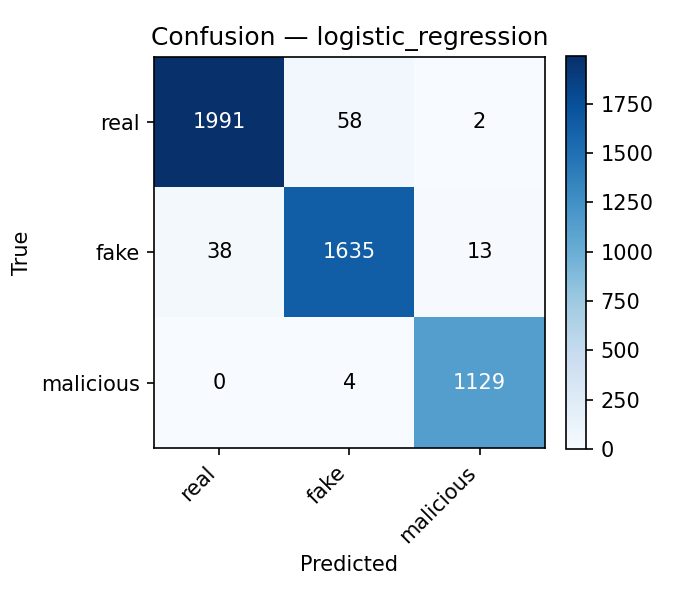
\includegraphics[width=0.6\linewidth]{reports/confusion_classical.png}
  \caption{Confusion matrix of the best classical model (Logistic Regression) on
  the held-out test split.}
  \label{fig:confusion}
\end{figure}

\subsection{Effect of the Fusion Modules}
Qualitative pipeline runs illustrate the value of fusion. A clickbait headline
with no source URL is driven toward a high-risk label by the writing-style module
when the classifier alone is uncertain; a phishing message receives compounding
risk from both the classifier and the scam-phrase detector; and a benign report
from a trusted domain is pulled toward \emph{real} by the credibility module.
Because unavailable modules are removed and their weight redistributed, the final
confidence remains calibrated whether or not a URL or external API is present.

\section{Conclusion}
The evaluation shows that the classical baselines already achieve strong
performance (best macro-F1 $0.978$), with the \emph{malicious} class detected
near-perfectly and the real-versus-fake boundary as the main source of error. The
transformer results (to be added from the Colab fine-tuning run) are expected to
narrow this gap further by modelling context, and the fusion modules add
provenance and corroboration signals that a content-only classifier cannot
capture.
